\documentclass[conference]{IEEEtran}
\usepackage{cite}
\usepackage{amsmath,amssymb}
\usepackage{graphicx}
\usepackage{booktabs}
\usepackage{tikz}
\usetikzlibrary{arrows.meta,positioning,calc}
\usepackage{url}
\usepackage{textcomp}
\def\BibTeX{{\rm B\kern-.05em{\sc i\kern-.025em b}\kern-.08em T\kern-.1667em\lower.7ex\hbox{E}\kern-.125emX}}

\begin{document}

\title{PI-CycleEV: Physics-Informed CycleGAN for Unpaired Summer--Winter Translation of Electric-Vehicle Driving Data}

\author{\IEEEauthorblockN{Muhammad Muntazir (66305), Taskeen Fatima (66757), Arooj Fatima (66703)}
\IEEEauthorblockA{Department of Computer Science, BUITEMS\\
Course: Machine Learning (Fall 2026), Instructor: Ms. Poma Panezai\\
Code: \url{https://github.com/MuntazirMalik/PI-CycleEV-Project}}}

\maketitle

\begin{abstract}
Synthetic multivariate time series can supplement scarce electric-vehicle (EV) driving data, but the state-of-the-art TS-p2pGAN needs paired signals. We reproduce TS-p2pGAN at a reduced training budget on the BMW~i3 real-driving dataset (70 trips) and propose PI-CycleEV, an unpaired 1D CycleGAN that translates driving windows between summer and winter and adds three physics-informed losses: Coulomb-counting SOC--current consistency, velocity--acceleration consistency and a window-level plausibility penalty. We evaluate on held-out trips with a trip-level split, using paired error, distribution, correlation, diversity, physics-residual and downstream SOC-estimation metrics, and an ablation of each physics term. The physics terms do what they are designed to do: the SOC residual falls from 18.4 (standard CycleGAN) to 0.0025 for summer-to-winter translation, and removing the velocity--acceleration term raises that residual from 2.7 to 72.3. However, physical consistency does not imply realism. PI-CycleEV reaches its low SOC residual with windows whose mean current ($-1.1$\,A against $-21.8$\,A in real data) and SOC change are close to zero, produced by large oscillations around zero and not by realistic driving, it does not improve fidelity over the standard CycleGAN, and both CycleGANs produce nearly constant window averages (diversity ratio 0.00--0.34, against about 1 for real data). As a data augmentation for SOC estimation, PI-CycleEV gives the lowest error of the augmentation methods in one direction (13.4 against 17.4 SOC points without augmentation) and no clear benefit in the other, with seed variance as large as the effects. We report these as negative and mixed results, together with all limitations of our single-run, reduced-budget study.
\end{abstract}

\begin{IEEEkeywords}
generative adversarial networks, CycleGAN, physics-informed learning, electric vehicles, time-series synthesis, state of charge
\end{IEEEkeywords}

\section{Introduction}
Data-driven models for EV energy management, such as state-of-charge (SOC) and motor-torque estimators, need driving data that cover many conditions, yet logging real trips is slow and expensive. Generative adversarial networks (GANs) \cite{goodfellow2014gan} can synthesize additional time series. Jeng \cite{jeng2025} proposed TS-p2pGAN, a pix2pix-style conditional GAN \cite{isola2017pix2pix} that generates SOC, battery voltage, motor torque and longitudinal acceleration from ten conditioning signals and reported realistic outputs on the BMW~i3 data. The paper itself names the reliance on paired data as a limitation and suggests unpaired CycleGAN architectures \cite{zhu2017cyclegan} augmented with physics-informed constraints as future work.

This project follows that suggestion. Our contributions are:
\begin{itemize}
\item a reduced-budget reproduction of TS-p2pGAN under a stricter, trip-level split (E1);
\item PI-CycleEV, an unpaired summer$\leftrightarrow$winter 1D CycleGAN with three physics-informed losses (E3), and a standard CycleGAN control (E2);
\item an evaluation that separates level from shape error and measures diversity, physics residuals and downstream SOC estimation (E4--E7), plus an ablation of each physics term;
\item an honest analysis showing where physics-informed training helps (physical consistency) and where it does not (fidelity, diversity, and the realism of generated magnitudes).
\end{itemize}

\section{Related Work}
\textbf{Conditional and cycle-consistent GANs.} Pix2pix \cite{isola2017pix2pix} learns a mapping from paired examples, which is the basis of TS-p2pGAN. CycleGAN \cite{zhu2017cyclegan} removes the need for pairs by adding a cycle-consistency loss; we follow its generator/discriminator design, with least-squares adversarial losses \cite{mao2017lsgan}, instance normalization \cite{ulyanov2016instance} and an identity loss.

\textbf{Time-series GANs.} TimeGAN \cite{yoon2019timegan} is a general time-series generator, and TS-p2pGAN \cite{jeng2025} reports better accuracy than it on EV driving data. Both rely on the training data being matched to the conditioning signals or to a single domain.

\textbf{Physics-informed learning.} Physics-informed neural networks \cite{raissi2019pinn} add residuals of known equations to the loss. We apply the same idea to GAN outputs, using battery charge conservation and kinematics. Our results show a limitation of this approach: a loss that only enforces a relation between signals can be satisfied by signals that are physically meaningless in magnitude.

\section{Data and Preprocessing}
We use the \emph{Battery and Heating Data for Real Driving Cycles} dataset \cite{ieeedata}: 70 trips of a BMW~i3 (60\,Ah), 32 in summer and 38 in winter, logged at 10\,Hz with 14 channels (10 conditioning signals and the four targets SOC, voltage, torque and acceleration). Each trip was cleaned (missing heater columns filled, trailing samples trimmed), smoothed with a ten-point moving average and downsampled to 1\,Hz. We scale every channel to $[-1,1]$ with a scaler fitted on training trips only, and cut windows of 256\,s with a stride of 4\,s.

\textbf{Trip-level split.} Trips, not windows, are split 70/15/15 (seed 42), so that no window of a test trip is seen in training (Table~\ref{tab:split}). This is stricter than evaluating on overlapping windows from the same trips, and it makes our baseline numbers not directly comparable with those in \cite{jeng2025}. The test set contains only five trips per season, so all test metrics have high variance.

\begin{table}[t]
\caption{Trip-level split and number of 256\,s windows.}
\label{tab:split}
\centering\small
\setlength{\tabcolsep}{3.5pt}
\begin{tabular}{lcccccc}
\toprule
 & \multicolumn{3}{c}{Trips} & \multicolumn{3}{c}{Windows}\\
\cmidrule(lr){2-4}\cmidrule(lr){5-7}
Season & Train & Val & Test & Train & Val & Test\\
\midrule
Summer & 22 & 5 & 5 & 5,823 & 1,956 & 1,886\\
Winter & 27 & 6 & 5 & 9,229 & 1,609 & 1,667\\
\bottomrule
\end{tabular}
\end{table}

\section{Method}
\subsection{Baseline (E1)}
We reimplemented TS-p2pGAN: a convolutional encoder, residual blocks and a transposed-convolution decoder with a two-scale discriminator, mapping the ten conditioning signals to the four targets. It was trained with Adam (learning rate $6\times10^{-4}$, linearly decayed from about epoch 38 of 50), batch size 256 and an L1 weight of 100 (our choice; the value is not given in \cite{jeng2025}). The original used 800 epochs; this reduced budget is a main limitation (Section~\ref{sec:limits}).

\subsection{PI-CycleEV (E3) and the CycleGAN control (E2)}
Two generators $G_{S\rightarrow W}$ and $G_{W\rightarrow S}$ translate complete 14-channel windows between seasons, and two PatchGAN discriminators judge realism in each season. Each generator is a 1D convolutional encoder (three stride-2 stages), six residual blocks with 64 base filters, and a transposed-convolution decoder with a $\tanh$ output; normalization is per-window instance normalization over the time axis. The generator objective is
\begin{equation}
\mathcal{L}_G=\mathcal{L}_{adv}+\lambda_{cyc}\mathcal{L}_{cyc}+\lambda_{id}\mathcal{L}_{id}+\lambda_{s}\mathcal{L}_{soc}+\lambda_{v}\mathcal{L}_{va}+\lambda_{r}\mathcal{L}_{rng},
\end{equation}
with least-squares adversarial loss, $\lambda_{cyc}=10$ and $\lambda_{id}=5$. E2 sets $\lambda_s=\lambda_v=\lambda_r=0$; E3 uses $(0.4,\,0.03,\,5.0)$, which are untuned starting values. We trained with Adam (learning rate $2\times10^{-4}$, $\beta_1=0.5$, constant), batch size 256, for 100 epochs (Fig.~\ref{fig:pipe}).

\begin{figure}[t]
\centering
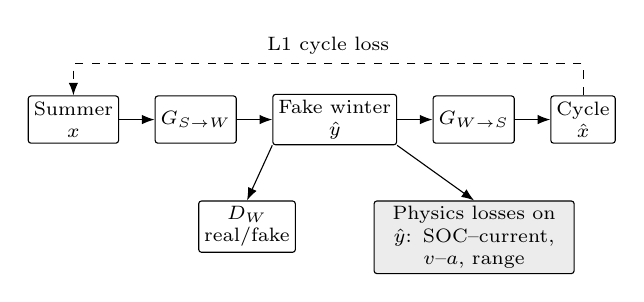
\begin{tikzpicture}[font=\scriptsize, node distance=3.2mm and 4.5mm,
 box/.style={draw,rounded corners=1pt,align=center,inner sep=2pt,minimum height=6mm},
 arr/.style={-{Latex[length=1.6mm]},thin}]
\node[box] (s) {Summer\\ $x$};
\node[box,right=of s] (g1) {$G_{S\rightarrow W}$};
\node[box,right=of g1] (w) {Fake winter\\ $\hat y$};
\node[box,right=of w] (g2) {$G_{W\rightarrow S}$};
\node[box,right=of g2] (c) {Cycle\\ $\hat x$};
\draw[arr] (s)--(g1); \draw[arr] (g1)--(w); \draw[arr] (w)--(g2); \draw[arr] (g2)--(c);
\node[box,below left=7mm and -3mm of w] (d) {$D_W$\\ real/fake};
\node[box,below right=7mm and -3mm of w,fill=gray!15,text width=24mm] (p) {Physics losses on $\hat y$: SOC--current, $v$--$a$, range};
\draw[arr] (w.south west)--(d.north); \draw[arr] (w.south east)--(p.north);
\draw[arr,dashed] (c.north) -- ++(0,4mm) -| (s.north) node[pos=.25,above]{L1 cycle loss};
\end{tikzpicture}
\caption{One direction of PI-CycleEV. The mirrored path (winter to summer) shares the same losses. Physics losses are computed on the generated window in physical units.}
\label{fig:pipe}
\end{figure}

\subsection{Physics-informed losses}
All physics terms are computed after converting the generated window back to physical units, and are normalized by reference values from real training windows (0 = consistent, about 1 = as bad as ignoring the physics).

\textbf{SOC--current (Coulomb counting).} Over a window of $T$ samples with step $\Delta t=1$\,s and capacity $C=60$\,Ah,
\begin{equation}
\Delta \mathrm{SOC}_I=\frac{100}{3600\,C}\sum_{t=1}^{T-1}\frac{I_t+I_{t+1}}{2}\Delta t,
\end{equation}
\begin{equation}
\mathcal{L}_{soc}=\frac{\mathbb{E}\big[(\mathrm{SOC}_T-\mathrm{SOC}_1-\Delta \mathrm{SOC}_I)^2\big]}{\mathrm{SOC}_{ref}},
\end{equation}
with negative current meaning discharge (checked on the data) and $\mathrm{SOC}_{ref}=8.72$.

\textbf{Velocity--acceleration.} With $v$ in km/h and $a_{ref}=0.3742$ (m/s$^2$)$^2$,
\begin{equation}
\mathcal{L}_{va}=\frac{\mathbb{E}\big[\big(\tfrac{v_{t+1}-v_t}{3.6\,\Delta t}-a_{t+1}\big)^2\big]}{a_{ref}}.
\end{equation}

\textbf{Plausibility.} $\mathcal{L}_{rng}$ penalizes SOC outside $[0,100]$\,\%, negative speed, and window averages or window SOC change outside the band spanned by the 1st--99th percentile of real training windows (window SOC change $-7.9$ to $-0.1$ points, mean current $-68.8$ to $-1.7$\,A). The window-level part was added during development after an earlier configuration produced self-consistent but absurd windows (for example a $-230$\,A average current).

\subsection{Evaluation protocol}
Test windows come only from held-out trips. \emph{Paired} metrics (RMSE, MAE and DTW \cite{senin2008dtw}, in \% of each signal's range) are computed only where a counterpart exists: E1 against its paired targets, and cycle and identity reconstructions for the CycleGANs. For the unpaired translations we compare \emph{distributions} with the mean, standard-deviation and Wasserstein differences (\% of range), the difference of correlation matrices among the four targets, a \emph{diversity ratio} (spread of window averages, generated over real; about 1 is as varied as real data, near 0 is collapsed), and the physics residuals. We also split each paired error into a per-window \emph{level} part and a within-window \emph{shape} part, where a flat prediction defines the shape error a model must beat.

\textbf{Metric definitions.} Let $r$ and $s$ be a real and a synthetic window of one signal, scaled to $[-1,1]$ (so halving an error gives a fraction of the signal's range), and $\bar r$, $\bar s$ their means over the window. The level and shape errors are
\begin{equation}
e_{level}=\mathbb{E}\,\tfrac{1}{2}\lvert\bar r-\bar s\rvert,\qquad
e_{shape}=\mathbb{E}\,\tfrac{1}{2}\lvert (r-\bar r)-(s-\bar s)\rvert,
\end{equation}
and the flat reference is $e_{flat}=\mathbb{E}\,\tfrac{1}{2}\lvert r-\bar r\rvert$, the shape error of a prediction that is constant within each window; a model captures within-window dynamics only if $e_{shape}<e_{flat}$. The diversity ratio of a signal is the standard deviation over windows of $\bar s$ divided by that of $\bar r$. Wasserstein and mean/standard-deviation differences are computed on all samples in physical units and divided by the signal's range. The correlation difference is the mean absolute difference of the off-diagonal entries of the correlation matrices of the four target signals. Errors are reported in \% of range.

\textbf{Downstream task (E4--E7).} A small SOC estimator (16,161 parameters; inputs current, voltage, battery and ambient temperature) is trained for 2,000 steps on real source-season windows (E4), plus an equal number of synthetic windows from TS-p2pGAN (E5), the standard CycleGAN (E6) or PI-CycleEV (E7), in both directions, and tested on real target-season test windows. A reference trained on real target-season data is an upper bound. Each setting uses three seeds. Because the baseline cannot translate seasons, E5 re-predicts the four outputs from real \emph{source}-season inputs.


\subsection{Experiments and settings}
Table~\ref{tab:exps} lists the experiments and Table~\ref{tab:hyper} the settings of the two model families. Every model was trained once with seed 42 on the same windows, the same trip split and the same scaler.

\begin{table}[t]
\caption{Experiments.}
\label{tab:exps}
\centering\small
\setlength{\tabcolsep}{3pt}
\begin{tabular}{lp{6.2cm}}
\toprule
ID & Description\\
\midrule
E1 & TS-p2pGAN baseline (paired)\\
E2 & Standard CycleGAN, all physics weights 0\\
E3 & PI-CycleEV, physics weights $(0.4,\,0.03,\,5.0)$\\
E4 & SOC estimator on real source-season windows only\\
E5 & E4 plus TS-p2pGAN windows\\
E6 & E4 plus standard-CycleGAN windows\\
E7 & E4 plus PI-CycleEV windows\\
Ablations & E3 without the SOC--current term, without the velocity--acceleration term, or without the range term\\
\bottomrule
\end{tabular}
\end{table}

\begin{table}[t]
\caption{Settings of the baseline and the CycleGAN models.}
\label{tab:hyper}
\centering\small
\setlength{\tabcolsep}{3pt}
\begin{tabular}{lcc}
\toprule
 & Baseline (E1) & CycleGAN (E2, E3)\\
\midrule
Training data & paired windows & unpaired windows\\
Epochs & 50 & 100\\
Optimizer & Adam & Adam ($\beta_1=0.5$)\\
Learning rate & $6\times10^{-4}$, linear decay & $2\times10^{-4}$, constant\\
Batch size & 256 & 256\\
Adversarial loss & -- & least squares\\
Other loss weights & L1: 100 & cycle 10, identity 5\\
Normalization & -- & instance (per window)\\
Window / stride & 256\,s / 4\,s & 256\,s / 4\,s\\
Seed & 42 & 42\\
\bottomrule
\end{tabular}
\end{table}

\section{Results}
\subsection{Reconstruction fidelity}
Table~\ref{tab:paired} lists paired errors. The baseline is far more accurate, but its task (predicting outputs from the real inputs of the same trip) is easier than unpaired translation. Between the CycleGANs, E2 is better than or equal to E3 on every cycle and identity measure except winter identity DTW and MAE, where E3 is marginally lower (9.12 against 9.15 and 9.52 against 9.58). Training for 100 instead of 50 epochs helped both: E3's summer cycle MAE fell from 11.9 to 9.8 and E2's from 9.7 to 8.4 (earlier 50-epoch evaluation of the same configuration).

\begin{table}[t]
\caption{Paired errors (\% of range, mean over the four targets; lower is better).}
\label{tab:paired}
\centering\small
\setlength{\tabcolsep}{3.5pt}
\begin{tabular}{llccc}
\toprule
Model & Test & DTW & MAE & RMSE\\
\midrule
E1 baseline & paired & 5.23 & 5.35 & 7.50\\
\midrule
E2 CycleGAN & cycle summer & 7.99 & 8.44 & 12.04\\
 & cycle winter & 9.56 & 10.24 & 13.60\\
 & identity summer & 7.35 & 7.74 & 11.15\\
 & identity winter & 9.15 & 9.58 & 12.78\\
\midrule
E3 PI-CycleEV & cycle summer & 9.71 & 9.81 & 13.89\\
 & cycle winter & 9.91 & 10.35 & 14.00\\
 & identity summer & 9.08 & 9.12 & 12.97\\
 & identity winter & 9.12 & 9.52 & 12.87\\
\bottomrule
\end{tabular}
\end{table}

The level/shape split shows where the error comes from. In the cycle reconstruction, the SOC level error is 13.3\,\% (summer) and 20.3\,\% (winter) of range for E2, and 18.2\,\% and 20.1\,\% for E3; even the paired baseline has an SOC level error of 11.9\,\% (in the example summer window its predicted SOC is about 10 points below the real one, while torque and acceleration follow the real signals closely). In contrast, shape errors of torque and acceleration are below the flat-prediction bar for both CycleGANs (for example torque, winter cycle: 4.76 for E2 and 4.85 for E3 against a flat reference of 7.99), meaning that within-window dynamics are partly captured. The SOC shape error, however, stays above its flat reference (for example 1.98 against 0.82 for E2 in the summer cycle), and the levels, especially SOC, are not captured.

\subsection{Distribution, correlation and diversity}
Table~\ref{tab:dist} summarizes distribution results. Wasserstein distances are close between E2 and E3 (E3 is lower for summer$\rightarrow$winter, 7.86 against 8.16, and higher for winter$\rightarrow$summer, 7.84 against 6.51). E2 has the smaller mean difference and correlation difference, while E3 has the smaller standard-deviation difference. The earlier 50-epoch evaluation gave Wasserstein values of 12.3 and 8.7 for E3 and 8.9 and 6.7 for E2, so longer training closed most of the gap.

\begin{table}[t]
\caption{Distribution distance to the real target season (\% of range, mean over the four targets) and correlation difference. S$\rightarrow$W: summer to winter; W$\rightarrow$S: winter to summer.}
\label{tab:dist}
\centering\small
\setlength{\tabcolsep}{3pt}
\begin{tabular}{lcccc}
\toprule
Model (direction) & Mean diff. & Std diff. & Wasserstein & Corr. diff.\\
\midrule
E1 (paired) & 2.32 & 1.49 & 2.51 & 0.020\\
E2 (S$\rightarrow$W) & 2.94 & 7.64 & 8.16 & 0.273\\
E2 (W$\rightarrow$S) & 4.26 & 6.74 & 6.51 & 0.225\\
E3 (S$\rightarrow$W) & 4.26 & 6.79 & 7.86 & 0.485\\
E3 (W$\rightarrow$S) & 6.18 & 5.24 & 7.84 & 0.253\\
\bottomrule
\end{tabular}
\end{table}

Fig.~\ref{fig:dist} shows the winter feature histograms. Neither model reproduces the real distributions: E2 concentrates SOC around 57 points, E3 spreads it over two ranges (about 47 and 70--85), neither reproduces the spike at zero velocity (standstill), and E3's current has the charging mode mentioned above. In the PCA and t-SNE embeddings (Fig.~\ref{fig:emb}) generated windows are separated from real ones for both models; in PCA, E2's windows lie at the edge of the real cloud, while E3's form a small cluster far from it.

\begin{figure*}[t]
\centering
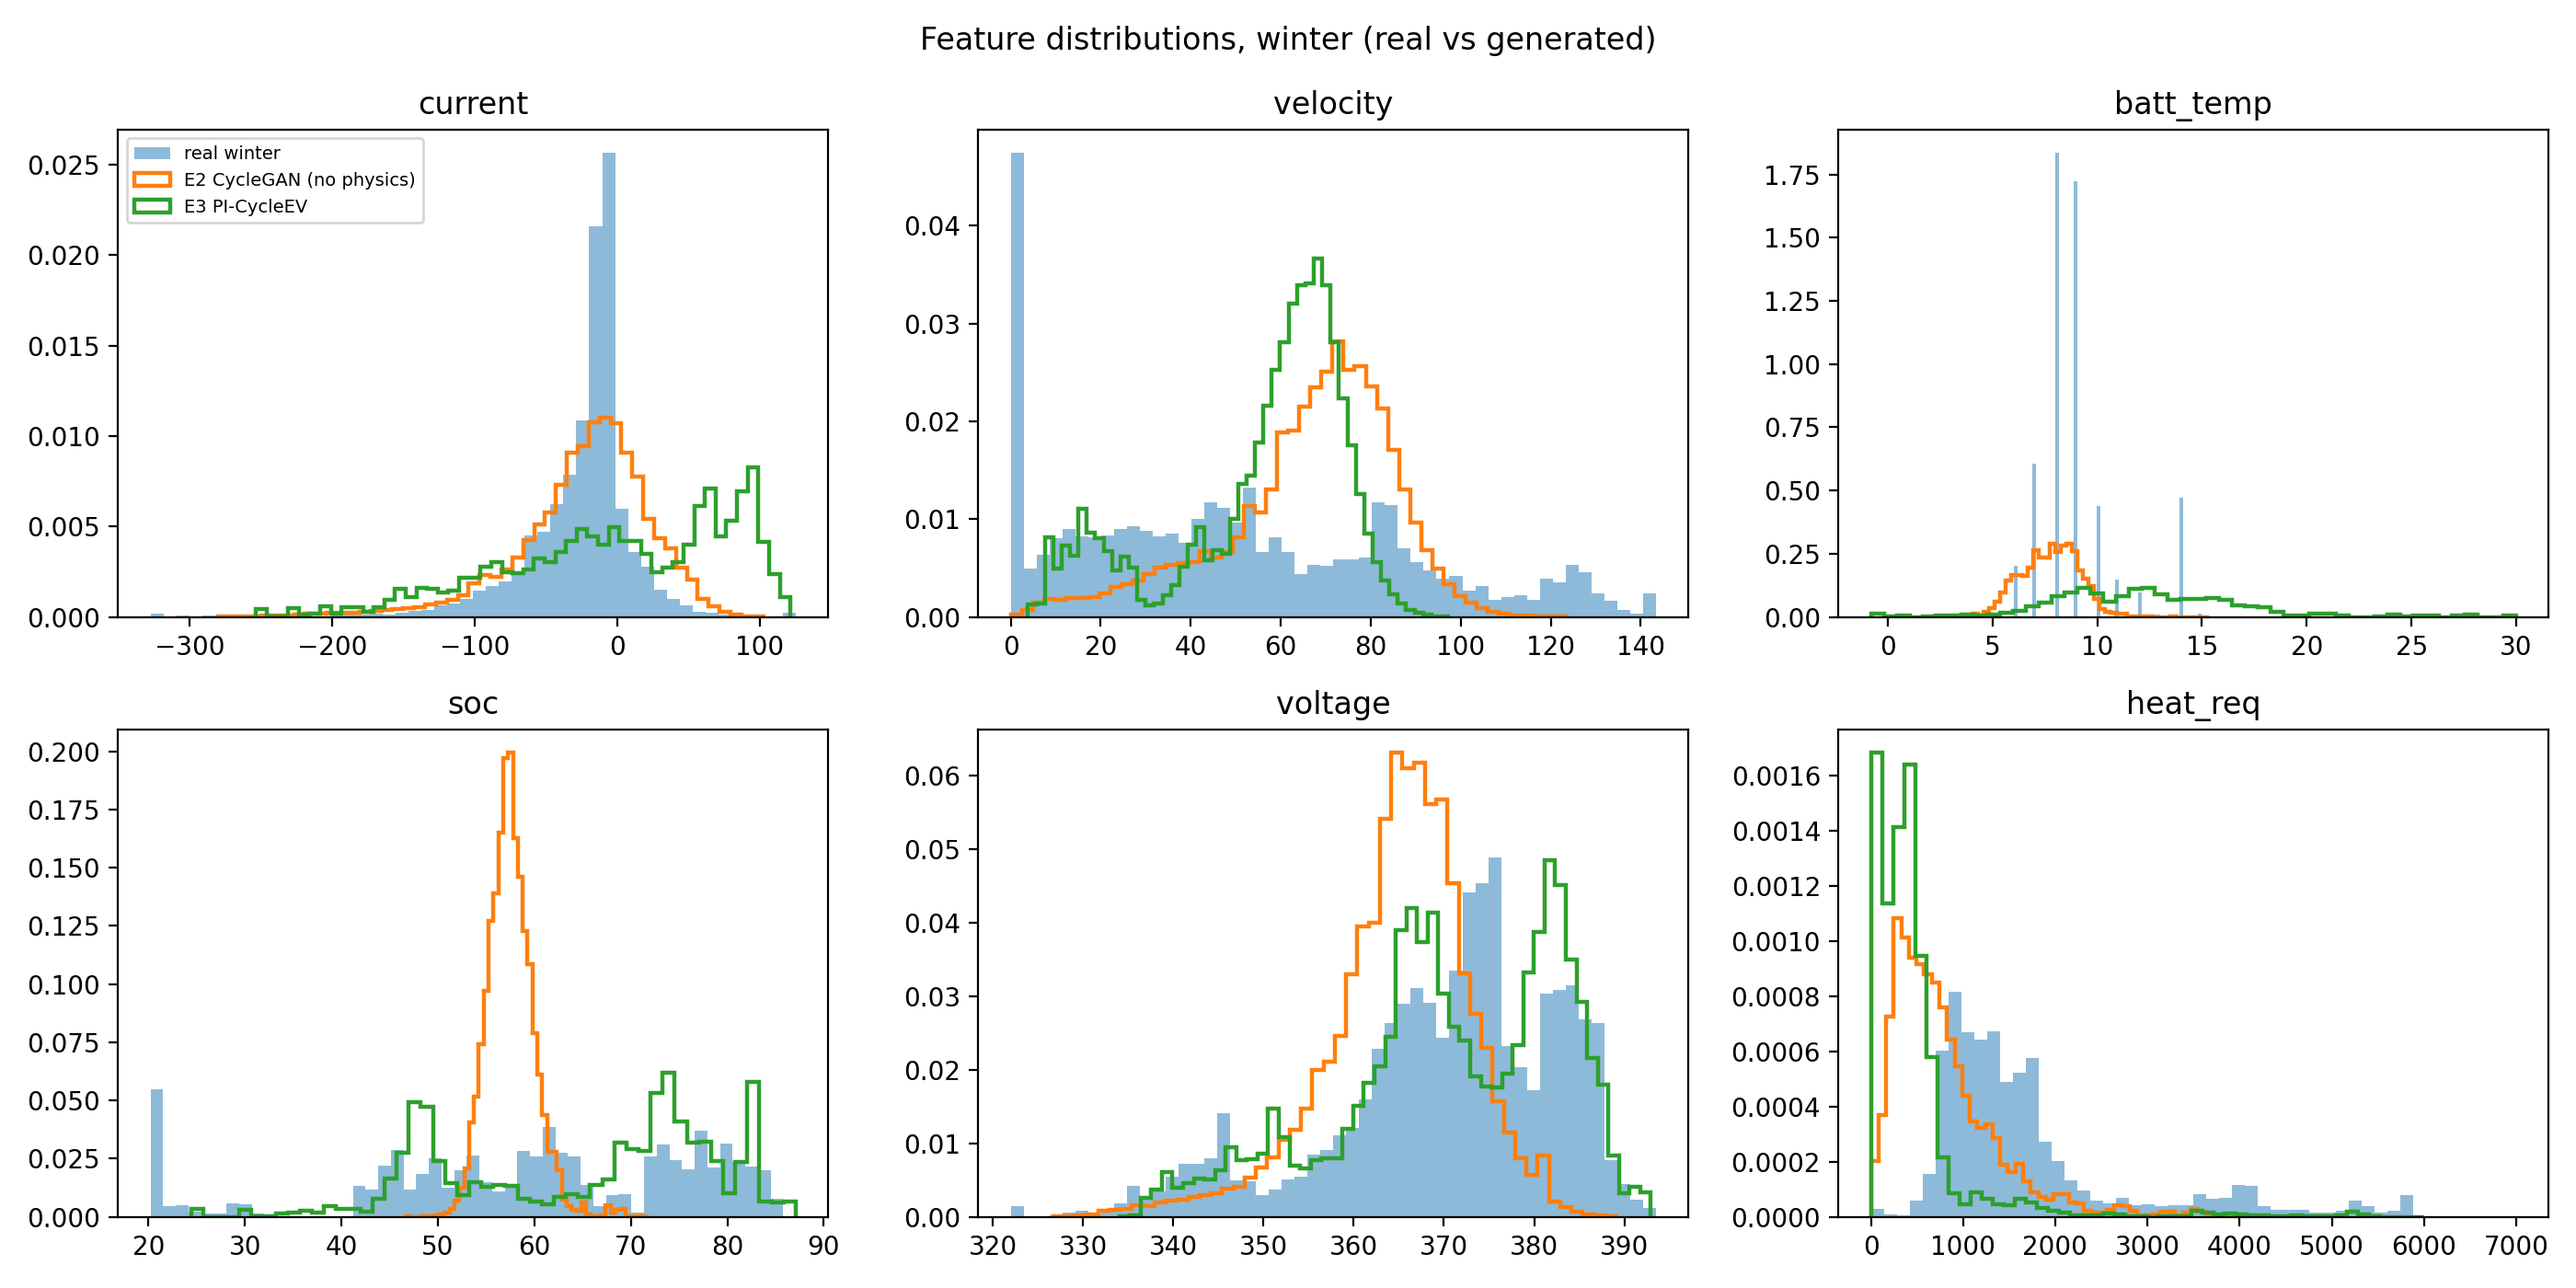
\includegraphics[width=0.92\textwidth]{figs/distributions_winter.png}
\caption{Feature histograms for winter: real test windows (filled) against E2 and E3 translations of summer test windows.}
\label{fig:dist}
\end{figure*}

\begin{figure*}[t]
\centering
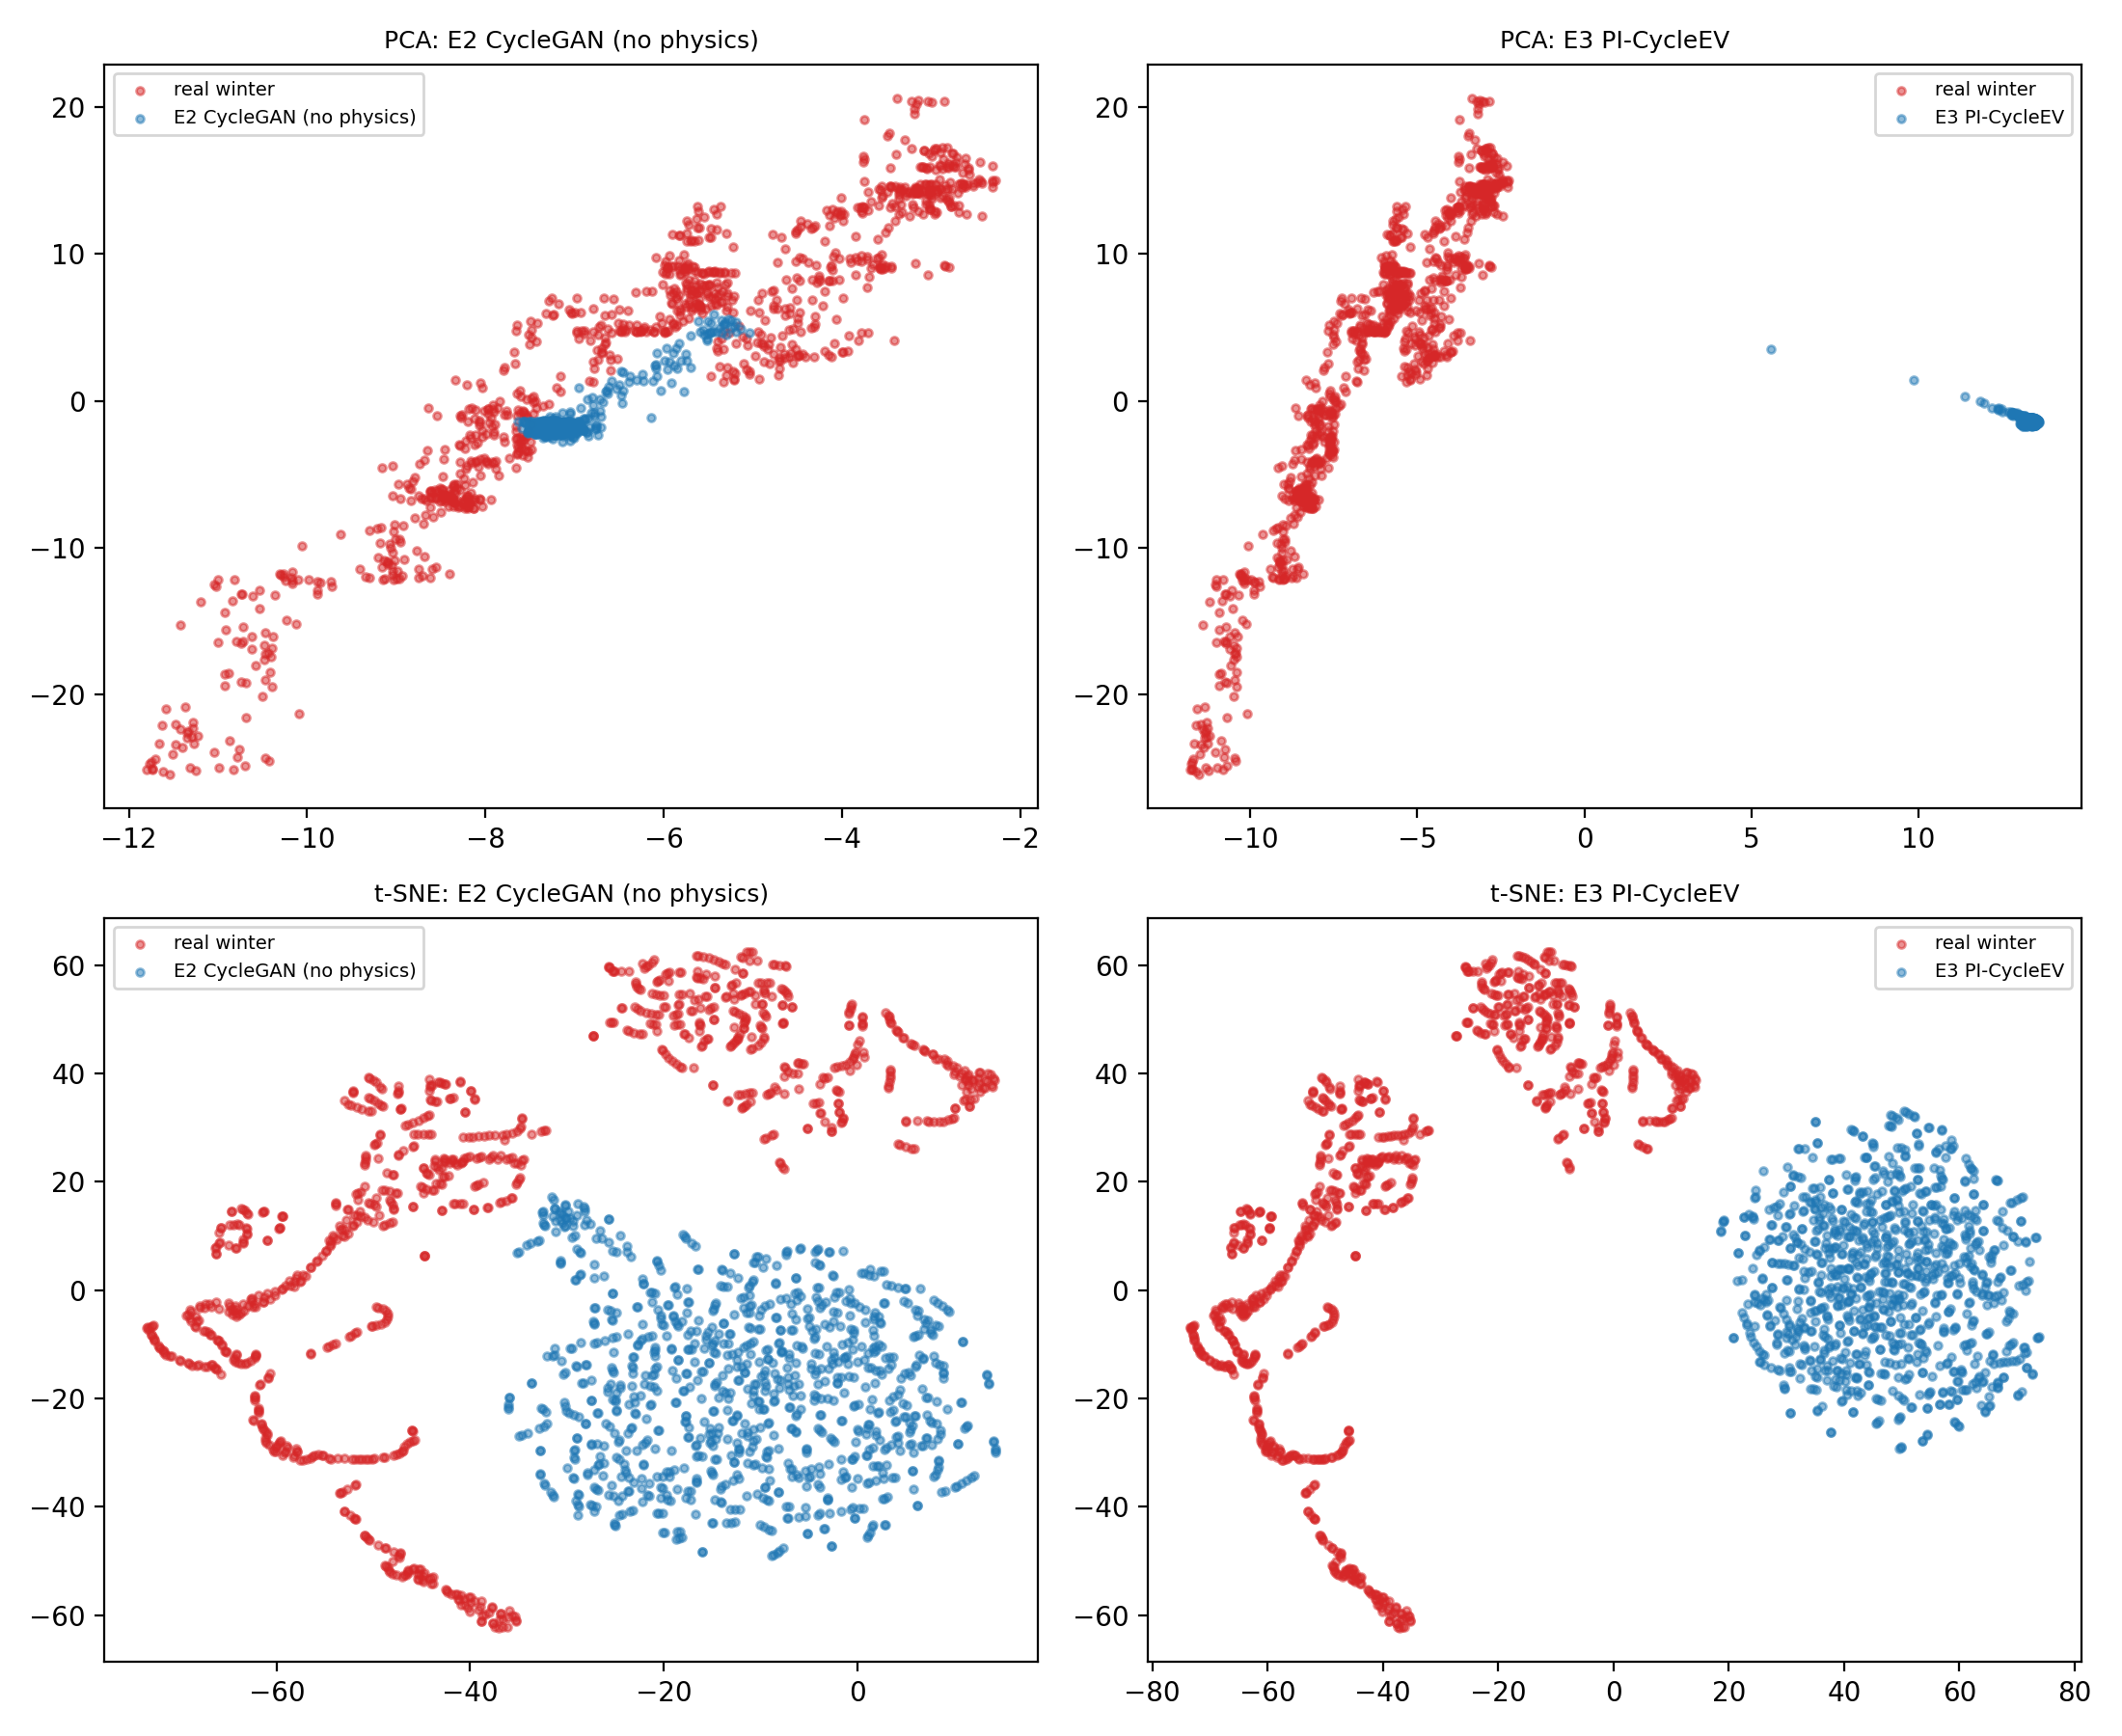
\includegraphics[width=0.62\textwidth]{figs/embedding_winter.png}
\caption{PCA (top) and t-SNE (bottom) of real winter windows and generated winter windows for E2 (left) and E3 (right).}
\label{fig:emb}
\end{figure*}

\textbf{Both CycleGANs collapse in diversity} (Table~\ref{tab:div}). Their generated window averages vary 0--34\,\% as much as real ones, whereas the paired baseline reaches 0.78--1.00. For E3, the summer$\rightarrow$winter SOC ratio is 0.00: all generated windows have the same average SOC. The distribution match in Table~\ref{tab:dist} is therefore achieved with little variation between windows.

\begin{table}[t]
\caption{Diversity ratio (spread of window averages, generated over real; about 1 is as varied as real data).}
\label{tab:div}
\centering\small
\setlength{\tabcolsep}{4pt}
\begin{tabular}{lcccc}
\toprule
Model (direction) & SOC & Voltage & Torque & Accel.\\
\midrule
E1 (paired) & 0.78 & 0.94 & 1.00 & 0.89\\
E2 (S$\rightarrow$W) & 0.03 & 0.14 & 0.25 & 0.34\\
E2 (W$\rightarrow$S) & 0.12 & 0.17 & 0.28 & 0.22\\
E3 (S$\rightarrow$W) & 0.00 & 0.02 & 0.11 & 0.07\\
E3 (W$\rightarrow$S) & 0.06 & 0.16 & 0.13 & 0.12\\
\bottomrule
\end{tabular}
\end{table}

As a diagnostic, we correlated the average of each channel in the input window with the average of the same channel in the generated window. For the four target channels the correlations lie between 0.01 and 0.61, while the input channels current, throttle and velocity are carried through much more strongly in winter$\rightarrow$summer (0.69--0.90). This is consistent with window-level information being only partly preserved, which may relate to the per-window normalization, but we did not test this explanation and treat it as a hypothesis.

\subsection{Physical consistency}
Table~\ref{tab:phys} shows that the physics terms work as designed. PI-CycleEV's SOC residual is 0.0025 (S$\rightarrow$W) and 0.0088 (W$\rightarrow$S), close to or below the real values (0.049 for winter and 0.0008 for summer), while the standard CycleGAN has 18.38 in the first direction. The velocity--acceleration residual is two to three times lower than for E2 (3.33 against 8.83, and 2.01 against 5.80), yet it remains an order of magnitude above the real value (0.18, 0.12).

\begin{table}[t]
\caption{Physics residuals (0 = consistent). Real test windows are the target.}
\label{tab:phys}
\centering\small
\setlength{\tabcolsep}{4pt}
\begin{tabular}{lcc}
\toprule
Model (direction) & SOC--current & Velocity--accel.\\
\midrule
E1 (paired) & 2.0241 & 0.1664\\
E2 (S$\rightarrow$W) & 18.3829 & 8.8302\\
E2 (W$\rightarrow$S) & 0.4315 & 5.8001\\
E3 (S$\rightarrow$W) & 0.0025 & 3.3302\\
E3 (W$\rightarrow$S) & 0.0088 & 2.0108\\
Real summer / winter & 0.0008 / 0.0490 & 0.1789 / 0.1245\\
\bottomrule
\end{tabular}
\end{table}

\textbf{Consistency is not realism.} The magnitude check in Table~\ref{tab:mag} and Fig.~\ref{fig:mag} shows how E3 achieves its low residual. The generated windows have a mean current of only $-0.2$\,A (S$\rightarrow$W) and $-2.1$\,A (W$\rightarrow$S), against $-25.5$ and $-18.1$\,A in the real target-season test windows, and their mean SOC change is $+0.1$ points against $-2.8$ and $-2.1$. Fig.~\ref{fig:ts} shows what this means in a typical window. E3's current swings between about $-250$ and $+120$\,A around a mean close to zero, its SOC jumps between about 35 and 85 points from one second to the next while starting and ending at the same value, and the other channels oscillate with a period of a few seconds as well. The SOC--current loss compares only the first and last SOC of a window with the integrated current, so such a window satisfies it by construction. E3's current histogram also has a second mode at $+50$ to $+120$\,A (Fig.~\ref{fig:dist}) that real winter driving does not have. The plausibility band does not prevent this: it constrains window averages and the endpoint SOC change, not the signal in between, and the upper edge of its band for the mean current ($-1.7$\,A) is close to zero. The standard CycleGAN's window is smooth and has a plausible current range, but its levels are wrong (its SOC stays at about 55--60 points), and over all summer$\rightarrow$winter windows its mean SOC change is $+10.2$ points while the current implies $-2.9$. These are single example windows and histograms, but they agree with the averaged numbers in Tables~\ref{tab:mag} and \ref{tab:abl}.

\begin{figure*}[t]
\centering
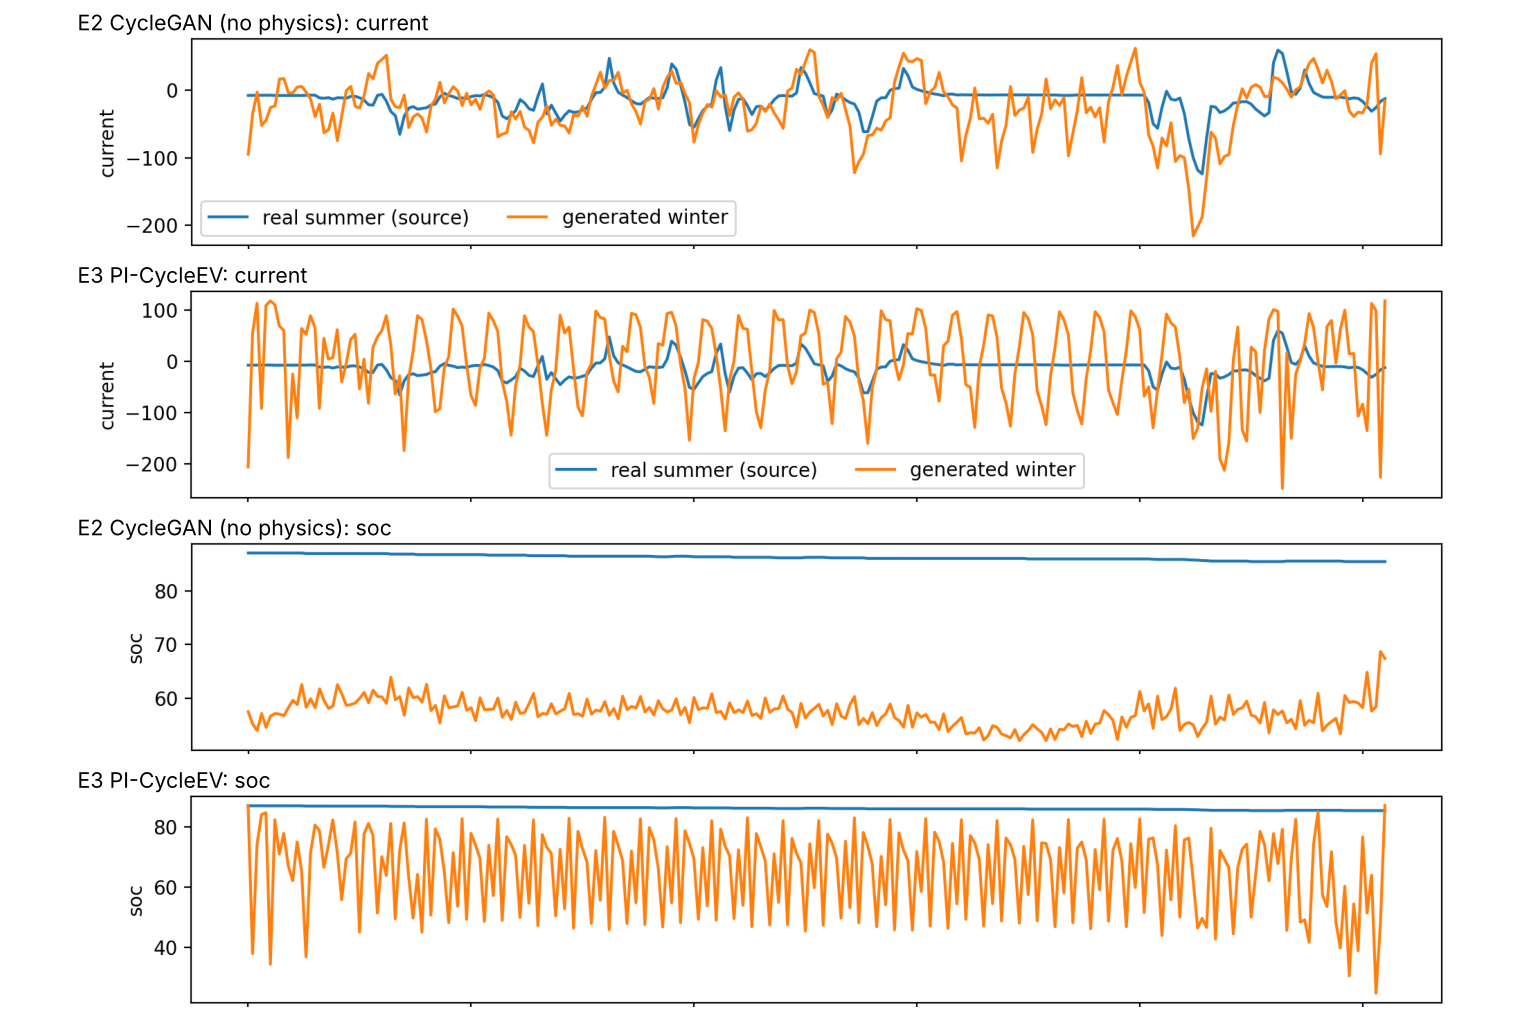
\includegraphics[width=\textwidth]{figs/timeseries_e2_e3.png}
\caption{The same summer test window translated to winter by E2 and by E3 (current and SOC; blue: real source window, orange: generated). Crops of the figures saved by the notebook.}
\label{fig:ts}
\end{figure*}

\begin{table}[t]
\caption{Magnitude check of the synthetic windows used in E5--E7 (per 256\,s window; units A and SOC points).}
\label{tab:mag}
\centering\small
\setlength{\tabcolsep}{3pt}
\begin{tabular}{lcccc}
\toprule
 & \multicolumn{2}{c}{S$\rightarrow$W} & \multicolumn{2}{c}{W$\rightarrow$S}\\
\cmidrule(lr){2-3}\cmidrule(lr){4-5}
Windows & Current & $\Delta$SOC & Current & $\Delta$SOC\\
\midrule
Real target test & $-25.5$ & $-2.8$ & $-18.1$ & $-2.1$\\
E5 TS-p2pGAN & $-15.8$ & $-2.1$ & $-25.8$ & $-2.0$\\
E6 CycleGAN & $-24.3$ & $+10.2$ & $-20.4$ & $-0.9$\\
E7 PI-CycleEV & $-0.2$ & $+0.1$ & $-2.1$ & $+0.1$\\
\bottomrule
\end{tabular}
\end{table}

\begin{figure}[t]
\centering
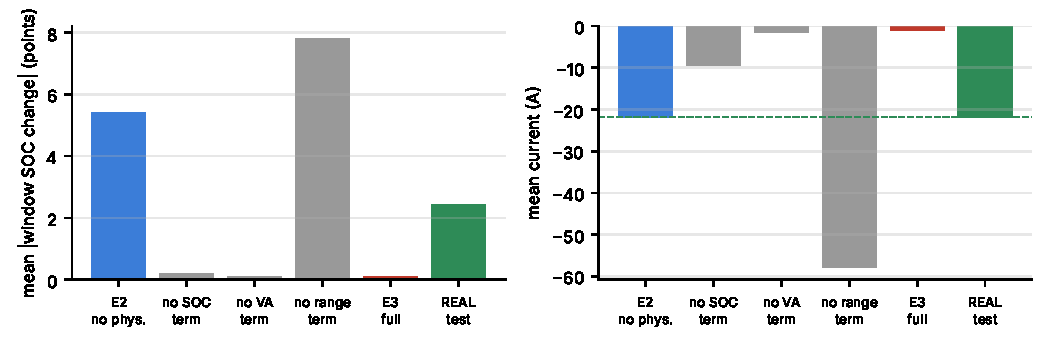
\includegraphics[width=\columnwidth]{figs/magnitude_check.pdf}
\caption{Ablation: mean absolute window SOC change and mean current of generated windows (both seasons averaged). The dashed line and the green bars are real test windows.}
\label{fig:mag}
\end{figure}

\subsection{Ablation of the physics terms}
Table~\ref{tab:abl} gives the ablation, each run trained once for 100 epochs. Removing a term makes its own residual worse: without the velocity--acceleration term its residual is 72.3 against 2.67; without the SOC term the SOC residual is 0.227 against 0.006, and the generated current falls to $-9.4$\,A. Without the range term the generated windows run away (mean current $-57.9$\,A, mean $|\Delta$SOC$|$ 7.8), so that term does constrain magnitude, while the full model, which includes it, ends at the other extreme ($-1.1$\,A). In Wasserstein distance the full model (7.85) is the best of the PI variants and close to E2 (7.34), while each removal costs 2.6--5.2 points. The cycle error in this table uses the pooled definition of the ablation cell and is therefore not comparable with Table~\ref{tab:paired}.

\begin{table}[t]
\caption{Ablation (averaged over both seasonal directions; Wasserstein and cycle RMSE in \% of range).}
\label{tab:abl}
\centering\small
\setlength{\tabcolsep}{2.6pt}
\begin{tabular}{lcccccc}
\toprule
Model & SOC res. & VA res. & $|\Delta$SOC$|$ & Current & Cycle RMSE & Wass.\\
\midrule
E2 (no physics) & 9.407 & 7.315 & 5.40 & $-21.9$ & 14.26 & 7.34\\
No SOC term & 0.227 & 1.926 & 0.20 & $-9.4$ & 18.28 & 13.02\\
No VA term & 0.014 & 72.326 & 0.11 & $-1.7$ & 18.14 & 11.97\\
No range term & 1.903 & 2.212 & 7.82 & $-57.9$ & 14.39 & 10.43\\
E3 (full) & 0.006 & 2.671 & 0.09 & $-1.1$ & 15.68 & 7.85\\
Real test & 0.025 & 0.152 & 2.43 & $-21.8$ & -- & --\\
\bottomrule
\end{tabular}
\end{table}

\subsection{Downstream SOC estimation}
Table~\ref{tab:down} and Fig.~\ref{fig:down} show the estimator's error on real target-season test windows. For summer$\rightarrow$winter, PI-CycleEV (E7) has the lowest mean RMSE of the augmentation methods, 13.4 against 17.4 without augmentation (E4), 20.3 for the baseline (E5) and 15.6 for the standard CycleGAN (E6); E7 is lower than E4 for two of the three seeds (not for seed~0: 12.6 against 11.4), and it has the highest $R^2$ (0.42) among them. The reference trained on real winter data reaches 4.6, so the gap to real data remains large. For winter$\rightarrow$summer no method helps convincingly. The mean of E4 (25.8) is dominated by one seed with RMSE 57.6; its median seed (13.8) is lower than that of E7 (15.6), and E5 (9.4) and E6 (11.0) are better than E7 (14.6), whose $R^2$ is negative ($-0.33$). With three seeds and standard deviations as large as the differences, we do not claim a significant effect. We also cannot attribute the one-direction gain to realism: Table~\ref{tab:mag} and Fig.~\ref{fig:ts} show that E7's windows oscillate by $\pm100$\,A around zero.

\begin{table}[t]
\caption{Downstream SOC estimation on real target-season test windows (SOC points; mean $\pm$ std over three seeds).}
\label{tab:down}
\centering\small
\setlength{\tabcolsep}{3pt}
\begin{tabular}{llccc}
\toprule
Direction & Training data & RMSE & MAE & $R^2$\\
\midrule
S$\rightarrow$W & E4 real only & $17.4\pm6.1$ & 14.8 & $-0.05$\\
 & E5 + TS-p2pGAN & $20.3\pm11.7$ & 18.9 & $-0.61$\\
 & E6 + CycleGAN & $15.6\pm2.0$ & 13.2 & 0.22\\
 & E7 + PI-CycleEV & $13.4\pm1.8$ & 9.8 & 0.42\\
 & Ref.\ real target & $4.6\pm0.2$ & 3.7 & 0.93\\
\midrule
W$\rightarrow$S & E4 real only & $25.8\pm27.8$ & 20.3 & $-6.19$\\
 & E5 + TS-p2pGAN & $9.4\pm1.7$ & 7.9 & 0.45\\
 & E6 + CycleGAN & $11.0\pm1.7$ & 7.3 & 0.25\\
 & E7 + PI-CycleEV & $14.6\pm2.5$ & 10.7 & $-0.33$\\
 & Ref.\ real target & $6.0\pm1.4$ & 4.0 & 0.78\\
\bottomrule
\end{tabular}
\end{table}

\begin{figure}[t]
\centering
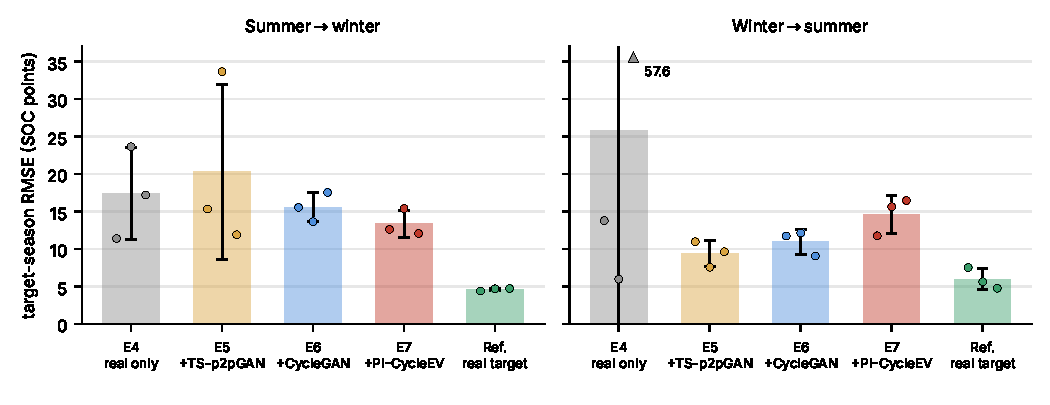
\includegraphics[width=\columnwidth]{figs/downstream_bars.pdf}
\caption{Target-season RMSE of the SOC estimator. Bars: mean over three seeds; whiskers: standard deviation; dots: individual seeds. The triangle marks one seed (57.6) outside the plotted range.}
\label{fig:down}
\end{figure}

\subsection{Development iterations}
The physics weights were not tuned for the reported results. During development we ran 10-epoch screens of the velocity--acceleration weight on the original architecture (Table~\ref{tab:screen}). Larger weights lowered that residual but increased the reconstruction loss and the SOC residual, so no setting dominated; we kept the starting value $\lambda_v=0.03$ for all reported runs. We also redesigned the SOC loss and added the window-level plausibility term during development, after configurations that produced implausible windows, and discarded earlier weights.

\begin{table}[t]
\caption{10-epoch screens of $\lambda_v$ (validation losses at epoch 10; not used for any reported result).}
\label{tab:screen}
\centering\small
\setlength{\tabcolsep}{4pt}
\begin{tabular}{lccc}
\toprule
$\lambda_v$ & Val.\ cycle & Val.\ SOC res. & Val.\ VA res.\\
\midrule
0.03 (control) & 0.519 & 0.038 & 7.78\\
0.1 & 0.541 & 0.040 & 3.48\\
0.3 & 0.556 & 0.052 & 1.48\\
1.0 & 0.585 & 0.077 & 1.05\\
3.0 & 0.631 & 0.143 & 0.87\\
\bottomrule
\end{tabular}
\end{table}

\section{Discussion}
Our results support a narrow claim and contradict a broad one. Physics-informed losses reliably reduce the residual of the relation they encode, and each term does what it names (Tables~\ref{tab:phys} and \ref{tab:abl}). They did not improve fidelity or diversity over the standard CycleGAN, and the lowest SOC residual was reached by shrinking current and SOC change toward zero, so the residual alone would have misled us about the model's quality. We therefore recommend reporting physics residuals together with magnitude checks against real windows, and with diversity.

\textbf{Why the residual can be satisfied trivially.} The SOC--current loss compares two quantities that are both generated: the change of the generated SOC between the first and the last sample, and the change implied by the generated current. A generator can reduce the difference by producing a current that integrates to about zero and a SOC that returns to its starting value, however much both oscillate in between (Fig.~\ref{fig:ts}); the loss never sees the intermediate samples. The plausibility band acts on window averages and on the same endpoint change, so it does not see them either. The ablation is consistent with this reading: without the range term the windows run away to $-57.9$\,A, and with it they sit at $-1.1$\,A, so the term bounds the average but does not place it near the real value ($-21.8$\,A). High-frequency oscillation of this kind is commonly associated with transposed-convolution upsampling, but we did not test that explanation. A loss on the per-step SOC increments or on within-window smoothness, a term tied to the real mean current, or conditioning the generator on window-level statistics would address the shortcut directly. We have not tested any of these.

\textbf{Diversity and level.} Both CycleGANs collapse to near-constant window averages, and the SOC level is poorly reproduced even by the paired baseline. A likely cause is that the level of a whole window is weakly constrained by unpaired adversarial and cycle losses, which act mainly on local structure; we did not verify a specific mechanism, and the window-mean diagnostic is only suggestive. Longer training helped (Tables~\ref{tab:paired} and \ref{tab:dist}), so part of the gap to the paper's 800-epoch baseline may be training budget.

\textbf{Downstream effect.} The summer$\rightarrow$winter gain of E7 is the one place where PI-CycleEV looks useful, but the evidence is thin. The estimator is trained with real current, voltage and temperature inputs, so windows whose current oscillates by $\pm100$\,A cannot represent realistic driving, and the gain may come from a shift in the SOC target distribution toward winter values and not from realism. The winter$\rightarrow$summer result, where nothing helps reliably, and the very large seed variance of the no-augmentation case argue against drawing a general conclusion. More seeds and a data-matched control (for example real windows from the target season at equal count) would be needed.

\textbf{Practical lessons.} Three choices mattered more than the architecture: the trip-level split (it removes optimistic window leakage, but leaves five test trips per season), the use of magnitude and diversity checks (they exposed failures that residuals and Wasserstein distances hid), and the training budget. A reproduction that is faithful in the loss design but short in epochs should be read as an indication, not as a measure of what the method can reach.

\section{Limitations}
\label{sec:limits}
\begin{itemize}
\item \textbf{Reduced budget:} the baseline was trained for 50 epochs (the original used 800) and the CycleGANs for 100, so the baseline and the CycleGANs do not have equal budgets, and our baseline does not reproduce the published accuracy.
\item \textbf{Single runs:} each model was trained once with one seed; no confidence intervals are available for the generators.
\item \textbf{Resumed runs:} E3 was continued from its epoch-70 checkpoint and the no-range ablation from epoch 20 after Colab sessions ended; only generators were restored, so discriminators and optimizers restarted.
\item \textbf{Small test set:} five test trips per season; downstream results use three seeds with standard deviations comparable to the effects.
\item \textbf{Untuned physics weights} and a baseline L1 weight chosen by us.
\item \textbf{Downstream design:} E5 uses source-season inputs because the baseline is paired; E4 is unstable across seeds.
\item \textbf{Metrics:} the ablation's cycle RMSE uses a different pooling than Table~\ref{tab:paired}.
\item \textbf{Content preservation:} nothing in the objective forces the generated velocity to follow the source trip; in the example window the generated velocity reaches about 100\,km/h (E2) and 78\,km/h (E3) against a source maximum below 60\,km/h.
\item \textbf{No realism test} beyond the measures above (for instance a trained real-versus-fake classifier).
\end{itemize}

\section{Conclusion}
We built an unpaired, physics-informed CycleGAN for summer--winter EV driving data and evaluated it against a reproduced paired baseline and a standard CycleGAN. The physics terms enforce what they encode, but they did not make the generated data more realistic, and they can be satisfied by oscillating windows whose mean current and endpoint SOC change are close to zero. The same model gave a downstream gain in one direction and none in the other, within the seed variance. Future work should add a magnitude-aware physics term or conditioning on window-level statistics, train for far longer, use several seeds, and test with a classifier-based realism measure.

\section*{Declaration of AI Use}
An AI assistant (Claude, Anthropic) was used for coding help, debugging and wording. All experiments were run by the authors and all reported numbers come from the saved outputs of those runs. [Confirm before submission.]

\begin{thebibliography}{00}
\bibitem{jeng2025} S.-L. Jeng, ``Generative adversarial network for synthesizing multivariate time-series data in electric vehicle driving scenarios,'' \emph{Sensors}, vol. 25, no. 3, Art. no. 749, 2025.
\bibitem{goodfellow2014gan} I. Goodfellow \emph{et al.}, ``Generative adversarial nets,'' in \emph{Proc. NIPS}, 2014, pp. 2672--2680.
\bibitem{isola2017pix2pix} P. Isola, J.-Y. Zhu, T. Zhou, and A. A. Efros, ``Image-to-image translation with conditional adversarial networks,'' in \emph{Proc. IEEE CVPR}, 2017, pp. 1125--1134.
\bibitem{zhu2017cyclegan} J.-Y. Zhu, T. Park, P. Isola, and A. A. Efros, ``Unpaired image-to-image translation using cycle-consistent adversarial networks,'' in \emph{Proc. IEEE ICCV}, 2017, pp. 2223--2232.
\bibitem{mao2017lsgan} X. Mao \emph{et al.}, ``Least squares generative adversarial networks,'' in \emph{Proc. IEEE ICCV}, 2017, pp. 2794--2802.
\bibitem{ulyanov2016instance} D. Ulyanov, A. Vedaldi, and V. Lempitsky, ``Instance normalization: The missing ingredient for fast stylization,'' arXiv:1607.08022, 2016.
\bibitem{raissi2019pinn} M. Raissi, P. Perdikaris, and G. E. Karniadakis, ``Physics-informed neural networks: A deep learning framework for solving forward and inverse problems involving nonlinear partial differential equations,'' \emph{J. Comput. Phys.}, vol. 378, pp. 686--707, 2019.
\bibitem{yoon2019timegan} J. Yoon, D. Jarrett, and M. van der Schaar, ``Time-series generative adversarial networks,'' in \emph{Proc. NeurIPS}, 2019.
\bibitem{senin2008dtw} P. Senin, ``Dynamic time warping algorithm review,'' Univ.\ Hawaii at Manoa, Honolulu, USA, Tech. Rep. 855, 2008.
\bibitem{ieeedata} ``Battery and heating data for real driving cycles,'' IEEE DataPort, 2022. [Online]. Available: https://ieee-dataport.org/open-access/battery-and-heating-data-real-driving-cycles
\end{thebibliography}

\end{document}
